\documentclass{iic2233activity}

\activitynumber{XX}
\semester{1}
\year{2020}
\activitydate{30 de Febrero} % Cambiar según actividad
\activitytitle{Template} % Cambiar según actividad
\pushtime{16:40} % Cambiar según actividad
% \evaluated{} % Comentar si no es evaluada
\formlink{---} % Cambiar para cada actividad no evaluada
\begin{document}

% BORRAR DESDE AQUÍ
\section*{Ideas}
\begin{itemize}
	\item Esta sección es para que vayan agregando ideas para la creación del enunciado de la AC, no importa si no están encargados de hacer esta AC. Cuando tengan la idea final borren esta sección.
\end{itemize}
% BORRAR HASTA AQUÍ

\section*{Introducción}

Aquí va una introducción breve sobre el  ``cuento'' de la actividad. Después de esta introducción no debería haber nada que distraiga a los alumnos.

La idea de la actividad es que sea lograble en el tiempo, y que puedan aprender lo que queremos que aprendan. En realidad este es un párrafo para rellenar el vacío de este documento, pero lo que dije es cierto. ¿Se dieron cuenta de que ahora \textbf{no} es necesario usar \texttt{`\textbackslash\textbackslash'} para cambiar de párrafo?

Para agregar una imagen, agrégala a la carpeta ``images'' y usa lo siguiente:

\begin{figure}[h!]
	\centering
	
\includegraphics[scale=0.4]{octocat.png}
\end{figure}

\clearpage % Lo usamos para crear una página nueva

También puedes poner dos imágenes, lado a lado:

\begin{figure}[h!]
	\centering
	\begin{subfigure}{.49\linewidth}
		\centering
		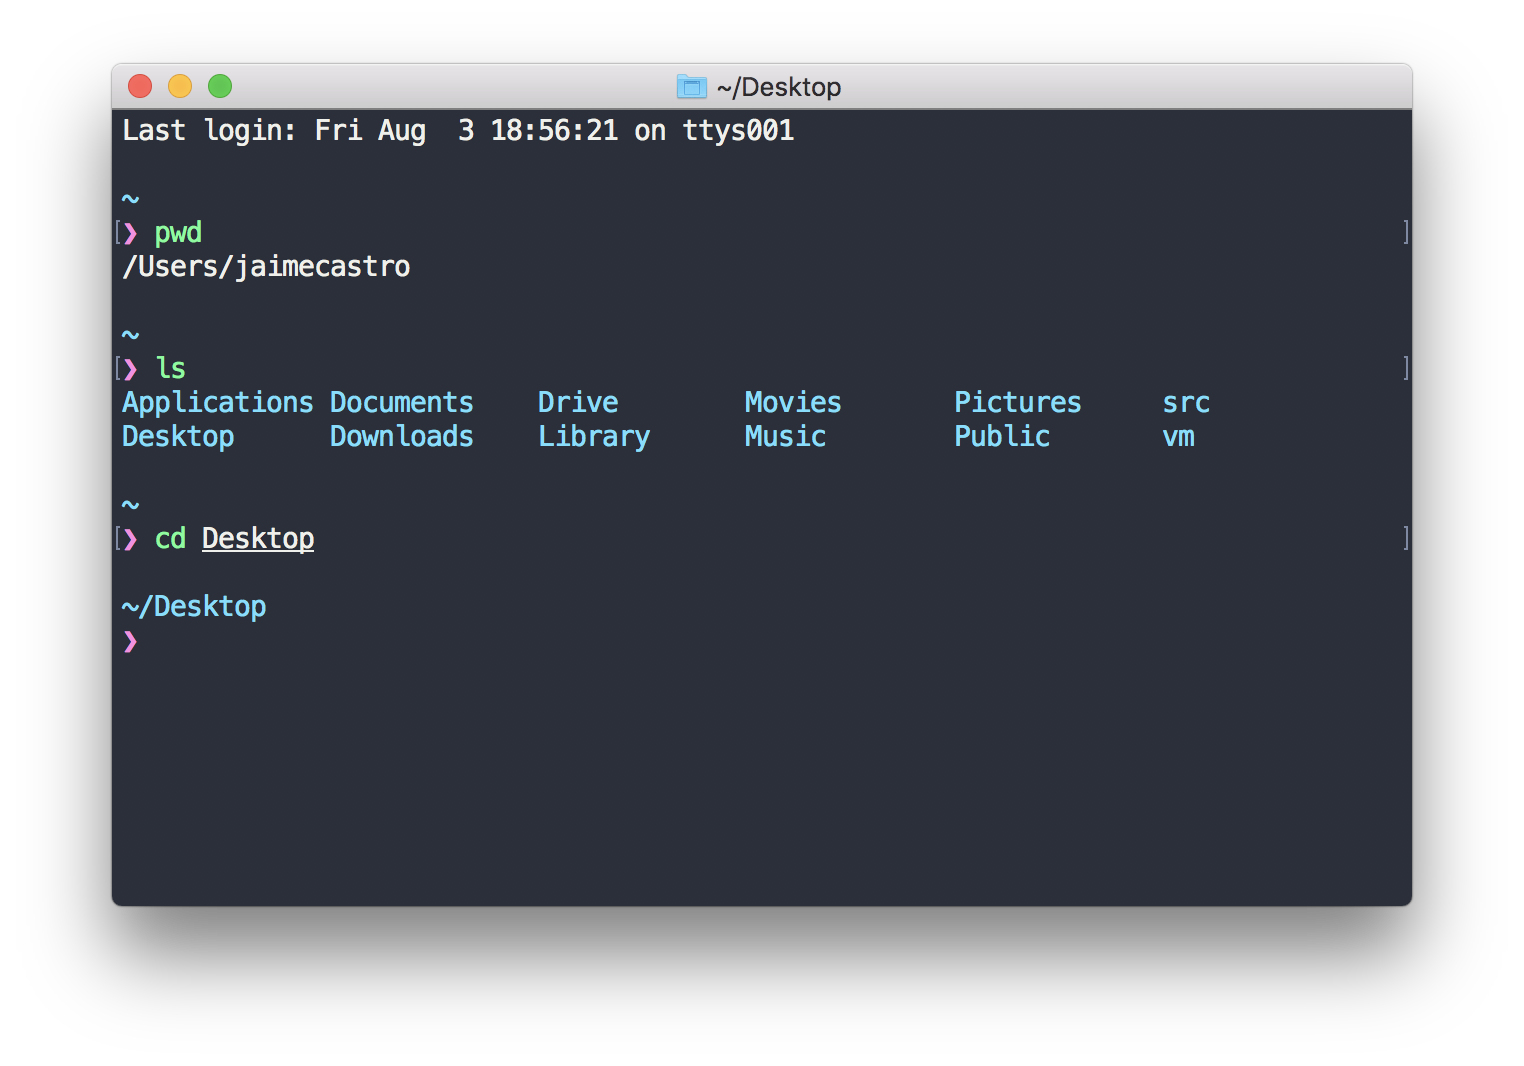
\includegraphics[height=5cm]{cd-mac.png}
	\end{subfigure}
	\begin{subfigure}{.49\linewidth}
		\centering
		
\includegraphics[height=5cm]{octocat.png}
	\end{subfigure}
\end{figure}

Podemos poder grandes pedazos de código, que incluso, viven en archivos de Python de verdad:

\pythoninput{code/sample.py}

\begin{python}
print('Este código está en el mismo LaTeX')
\end{python}


También podemos poner Python \textit{inline}: \mil{import solucion}.

\section*{Notas}

\begin{itemize}
	\item Aquí se pueden escribir consejos para desarrollar la actividad.
	\item También se pueden mencionar detalles importantes de la actividad, como alguna función no común de alguna librería a usar.
\end{itemize}

\section*{Requerimientos}
\begin{itemize}
	\item (3.00 pts) Primer requerimiento
	      \begin{itemize}
		      \item (1.50 pts) Primera parte del primer requerimiento
		      \item (1.50 pts) Segunda parte del primer requerimiento
	      \end{itemize}
	\item (3.00 pts) Segundo requerimiento
\end{itemize}

\end{document}